%% ============================================================
%%  Automated GRD Prediction — Hospital El Pino
%%  Camera-ready · IEEEtran journal class
%%  Compiler : pdfLaTeX  (Overleaf default)
%%  Build    : pdflatex → bibtex → pdflatex → pdflatex
%% ============================================================
\documentclass[journal]{IEEEtran}

%% ── Core typography & encoding
\usepackage[T1]{fontenc}
\usepackage[utf8]{inputenc}
\usepackage{microtype}

%% ── Math
\usepackage{amsmath,amssymb,amsfonts}

%% ── Graphics & colour
\usepackage{graphicx}
\usepackage{xcolor}

%% ── Tables
\usepackage{booktabs}
\usepackage{multirow}
\usepackage{array}
\usepackage{threeparttable}

%% ── Lists
\usepackage{enumitem}

%% ── References & links
\usepackage{cite}
\usepackage{url}
\usepackage[hidelinks,
            colorlinks=true,
            linkcolor=blue!60!black,
            citecolor=blue!60!black,
            urlcolor=blue!60!black]{hyperref}

%% ── Layout helpers
\usepackage{balance}

%% ── Figure path (all PNGs placed in ./figures/)
\graphicspath{{figures/}}

%% ============================================================
\begin{document}

\title{Automated GRD Prediction from Clinical Data Using\\
       Machine Learning: A Multi-Class Classification\\
       Approach for Hospital El Pino}

\author{Cristopher~Pradenas,~Mat\'ias~Al\'e,~and~Diego~Lobos~D\'iaz~Emiliano Fernandez~Felipe salas ortiz%
  \thanks{C.~Pradenas, M.~Al\'e, and D.~Lobos~D\'iaz are with
          the School of Engineering, Universidad Andr\'es Bello,
          Santiago, Chile (CINF104 Aprendizaje de M\'aquinas).
          E-mail: \texttt{\{[student-emails]\}@uandresbello.edu}.}%
  \thanks{Manuscript received [DD~Mon.\ YYYY]; revised
          [DD~Mon.\ YYYY]; accepted [DD~Mon.\ YYYY].}}

\maketitle

%% ── Abstract ─────────────────────────────────────────────────
\begin{abstract}
The automated assignment of \emph{Grupos Relacionados por el
Diagn\'ostico} (GRD) codes is indispensable for hospital
resource planning and healthcare financing under Chile's Fondo
Nacional de Salud (FONASA) reimbursement framework.  Manual
coding, however, remains labour-intensive and is inherently
susceptible to inter-coder variability.  We propose a supervised
machine learning framework to automate this process using
structured clinical data from Hospital El Pino, comprising
\textbf{14,561} inpatient episodes and \textbf{526} unique GRD
categories.  Our pipeline applies binary TF-IDF encoding to
CIE-10 diagnostic and CIE-9 procedural fields, yielding a
2,995-dimensional feature matrix with 99.28\,\% sparsity.
Four architectures---Logistic Regression, Random Forest,
XGBoost, and a Multilayer Perceptron (MLP)---were systematically
evaluated.  The MLP demonstrates superior discriminative
capability, achieving an accuracy of \textbf{0.8168} and a
macro-averaged F1-score of \textbf{0.7433} on the 80 most
frequent GRD classes, which collectively account for 70.8\,\%
of the dataset.  These results establish the viability of
automated, structured-data pipelines as low-latency
decision-support tools for clinical coding in Chilean public
hospitals.
\end{abstract}

\begin{IEEEkeywords}
GRD prediction, diagnosis-related groups, clinical coding
automation, multi-class classification, multilayer perceptron,
CIE-10, CIE-9, Hospital El Pino, high-dimensional sparsity,
binary TF-IDF encoding.
\end{IEEEkeywords}

%% ============================================================
\section{Introduction}
\label{sec:intro}
%% ============================================================

The \emph{Grupos Relacionados por el Diagn\'ostico} (GRD)
system constitutes a patient classification framework adapted
in Chile from the Diagnosis-Related Groups (DRG) methodology
developed in the United States~\cite{slee1978}.  FONASA employs
GRD codes to determine hospital reimbursement rates under the
\emph{Modalidad de Atenci\'on Institucional}~\cite{minsal2013},
rendering accurate code assignment a direct determinant of
hospital revenue and resource allocation.  In current clinical
practice, coding specialists retrospectively assign GRD labels
by reviewing principal and secondary diagnoses, procedures, and
discharge summaries---a process that is labour-intensive and
generates measurable inter-coder variability~\cite{goldstein2017}.
Automating this retrospective process through machine learning
has consequently emerged as a critical research priority for
reducing administrative overhead in healthcare
systems~\cite{baumel2018,perotte2014}.

This study frames automated GRD prediction as a supervised
multi-class classification problem defined on structured
patient-level data: CIE-10 diagnostic codes, CIE-9 procedural
codes, patient age, and biological sex.  The primary
computational challenges are three-fold: 526 unique GRD
categories distributed across an extreme imbalance ratio of
$813{:}1$; a feature space exhibiting 99.28\,\% sparsity; and
the unordered, multi-valued nature of the diagnostic and
procedural fields.  To address these challenges, we evaluate
four architectures---ranging from tree-based ensembles such
as XGBoost~\cite{chen2016} to feedforward neural networks---and
assess their capacity to extract discriminative clinical patterns
from this high-dimensional tabular
representation~\cite{che2018,mullenbach2018}.

The study is conducted on 14,561 inpatient records from Hospital
El Pino, Santiago, Chile, each episode described by up to 35
CIE-10 diagnostic codes and up to 30 CIE-9 procedural codes.
To ensure full reproducibility, the preprocessing pipeline,
model implementations, and trained artefacts are publicly
available at: \textbf{\url{[https://github.com/Cristxpherr/CINF104-GRD-HospitalElPino]}}. 
The remainder of this paper is structured as follows:
Section~\ref{sec:related} surveys related work;
Section~\ref{sec:objective} formulates the study objectives;
Section~\ref{sec:methodology} details the methodology;
Section~\ref{sec:eda} presents the exploratory data analysis;
Section~\ref{sec:results} reports experiments, results, and
discussion; Sections~\ref{sec:conclusions}
and~\ref{sec:limitations} state conclusions and limitations;
and Section~\ref{sec:availability} describes data and code
availability.

%% ============================================================
\section{Related Work}
\label{sec:related}
%% ============================================================

Building on Slee's foundational patient classification
framework~\cite{slee1978}, the automation of clinical coding
has evolved from natural language processing (NLP) applied to
free-text discharge summaries~\cite{perotte2014,baumel2018} to
predictive modelling on structured electronic health records
(EHRs).  This shift is primarily motivated by the quantifiable
economic impact of manual coding inconsistencies on hospital
revenue cycles~\cite{goldstein2017}.

For structured, tabular clinical data, gradient-boosted tree
ensembles such as XGBoost~\cite{chen2016} constitute highly
competitive baselines, benefiting from native support for sparse
feature matrices and built-in $L_1$/$L_2$ regularisation.
Nevertheless, when input representations attain extreme
dimensionality and sparsity---as is the case with multi-hot
ICD code encodings---feedforward neural architectures have
demonstrated superior capacity to distil latent clinical
representations that transcend the expressive limits of
tree-based splitting criteria~\cite{che2018}.

In the domain of automated DRG prediction, Janke
et~al.~\cite{janke2017} reported macro F1-scores of 0.70--0.82
on curated subsets of US hospital data using logistic regression
and random forests, while Boag et~al.~\cite{boag2018}
established the strong predictive value of clinical code
co-occurrence patterns from MIMIC-III.  Li et~al.~\cite{li2022}
proposed graph-based ICD code embeddings leveraging the
hierarchical ICD taxonomy, achieving accuracy above 0.85 on
curated MIMIC-III subsets.  In marked contrast, predictive GRD
modelling in Latin America remains scarce; regional literature
is predominantly oriented toward administrative cost
analysis~\cite{minsal2013}.  This study addresses that gap by
applying structured machine learning to a real-world Chilean
hospital cohort, navigating the compounded challenges of a
large-cardinality, severely imbalanced GRD label space and
99.28\,\% feature sparsity.

%% ============================================================
\section{Objective of the Study}
\label{sec:objective}
%% ============================================================

The primary objective is to develop and rigorously evaluate a
supervised machine learning model capable of automatically
predicting the GRD code for a patient hospitalization episode
from structured clinical data available at the time of discharge.
The following specific sub-objectives guide the investigation:

\begin{enumerate}[label=(\roman*), leftmargin=*, itemsep=2pt]
  \item To conduct a thorough exploratory data analysis (EDA)
        of the Hospital El Pino cohort, characterising data
        quality, class distribution, and discriminative feature
        properties.
  \item To design and implement a preprocessing and feature
        engineering pipeline that transforms sparse,
        multi-valued CIE-10 and CIE-9 code fields into a form
        amenable to standard classification algorithms.
  \item To train and compare multiple supervised learning
        architectures---Logistic Regression, Random Forest,
        XGBoost, and a Multilayer Perceptron---on the
        prediction task.
  \item To select the best-performing model according to
        macro-averaged classification metrics appropriate for
        the severely imbalanced label distribution.
  \item To contextualise the obtained results within the
        broader DRG/GRD prediction literature.
\end{enumerate}

%% ============================================================
\section{Methodology}
\label{sec:methodology}
%% ============================================================

\subsection{Dataset Description}

The dataset comprises 14,561 retrospective inpatient episodes
from Hospital El Pino, Santiago, Chile.  Demographic variables
include biological sex---female patients constitute a majority
of 66.0\,\% ($n{=}9{,}617$) versus 34.0\,\% male
($n{=}4{,}944$)---and age (mean\,=\,39.43 years,
$\mathrm{SD}{=}24.68$, median\,=\,36, IQR\,=\,23--60).  The
clinical trajectory for each episode is encoded via one
principal and up to 34 secondary \emph{CIE-10} diagnosis codes,
alongside one principal and up to 29 secondary \emph{CIE-9}
procedure codes.  Secondary fields display a missingness rate
of 81.8\,\% for diagnoses and 57.9\,\% for procedures---values
that reflect intrinsic variation in clinical complexity rather
than data entry deficiencies.  The target variable is the GRD
code, encompassing 526 unique categories with a class imbalance
ratio of $813{:}1$.  All records were de-identified prior to
analysis in compliance with patient privacy regulations.

\subsection{Development Method}

The pipeline initiates with rigorous data cleaning and text
normalisation.  Each compound code field of the form
\texttt{CODE\,--\,Description} is parsed to retain only the
alphanumeric prefix (e.g., \texttt{A41.8} from
\texttt{A41.8\,--\,Otras septicemias}).  Missing age values
are imputed with the training-set median.  To ensure stratified
splitting validity, 76 singleton GRD classes are removed,
yielding a final analytical corpus of \textbf{14,485} records
across \textbf{450} active GRD classes.  A stratified 80/20
partition produces 11,588 training records and 2,897 hold-out
test records, preserving the imbalanced clinical distribution
across both subsets.

\subsection{Machine Learning Techniques}
\label{sec:techniques}

Feature engineering transforms CIE-10 diagnostic codes and
CIE-9 procedural codes into a unified numerical representation
via binary TF-IDF vectorisation with
$\mathrm{min\_df}{=}2$.  The set of all principal and secondary
CIE-10 diagnosis codes per episode is concatenated as a bag of
tokens; an identical operation is applied to CIE-9 procedure
codes.  The two resulting binary matrices (2,365 diagnostic
features; 628 procedural features) are horizontally concatenated
with $z$-score-standardised age and binary-encoded sex,
producing the final \textbf{2,995-dimensional} feature matrix
(sparsity: \textbf{99.28\,\%}).

Four supervised learning architectures are evaluated:

\begin{itemize}[leftmargin=*, itemsep=2pt]
  \item \textbf{Logistic Regression (LR):} Multinomial
        classifier with $L_2$ regularisation ($C{=}1.0$,
        \textit{saga} solver), linear baseline suited to
        sparse binary matrices.
  \item \textbf{Random Forest (RF):} Bagging ensemble of
        100 decision trees ($\mathrm{max\_depth}{=}20$,
        $\mathrm{min\_samples\_leaf}{=}2$).
  \item \textbf{XGBoost:} Regularised gradient-boosted
        ensemble (80 estimators, $\mathrm{max\_depth}{=}5$,
        $\eta{=}0.15$, subsample\,=\,0.8)~\cite{chen2016}.
  \item \textbf{Multilayer Perceptron (MLP):} Two hidden
        layers (256 and 128 neurons), ReLU activations,
        $L_2$ regularisation ($\alpha{=}10^{-4}$), Adam
        optimiser ($\eta{=}10^{-3}$), batch size 512, and
        early stopping (patience\,=\,10) on a 10\,\% internal
        validation split.
\end{itemize}

\subsection{Evaluation Metrics}

The class imbalance ratio of $813{:}1$ renders overall accuracy
an inadequate primary metric, as it disproportionately rewards
correct classification of majority classes while masking
degraded performance on rare but clinically significant GRDs.
Accordingly, the \textbf{macro-averaged F1-score}---which
computes F1 independently per class and averages without
frequency weighting---is adopted as the principal optimisation
criterion.  Weighted F1-score and overall accuracy are
additionally reported.  A normalised confusion matrix restricted
to the top-12 GRD categories is analysed to identify systematic
misclassification patterns.

%% ============================================================
\section{Exploratory Data Analysis}
\label{sec:eda}
%% ============================================================

\subsection{Data Quality Assessment}

A systematic assessment establishes the dataset's integrity
prior to modelling.  As illustrated in
Fig.~\ref{fig:missingness}, both the principal CIE-10 diagnosis
field and the principal CIE-9 procedure field exhibit 0.0\,\%
missingness, providing a complete clinical baseline for every
episode.  Secondary fields display a monotonically increasing
missingness rate with column index, averaging 81.8\,\% for
CIE-10 secondary diagnoses and 57.9\,\% for CIE-9 secondary
procedures---an intrinsic characteristic of clinical coding
practice that validates the sparse vectorisation strategy
adopted in Section~\ref{sec:techniques}.

\begin{figure}[!t]
  \centering
  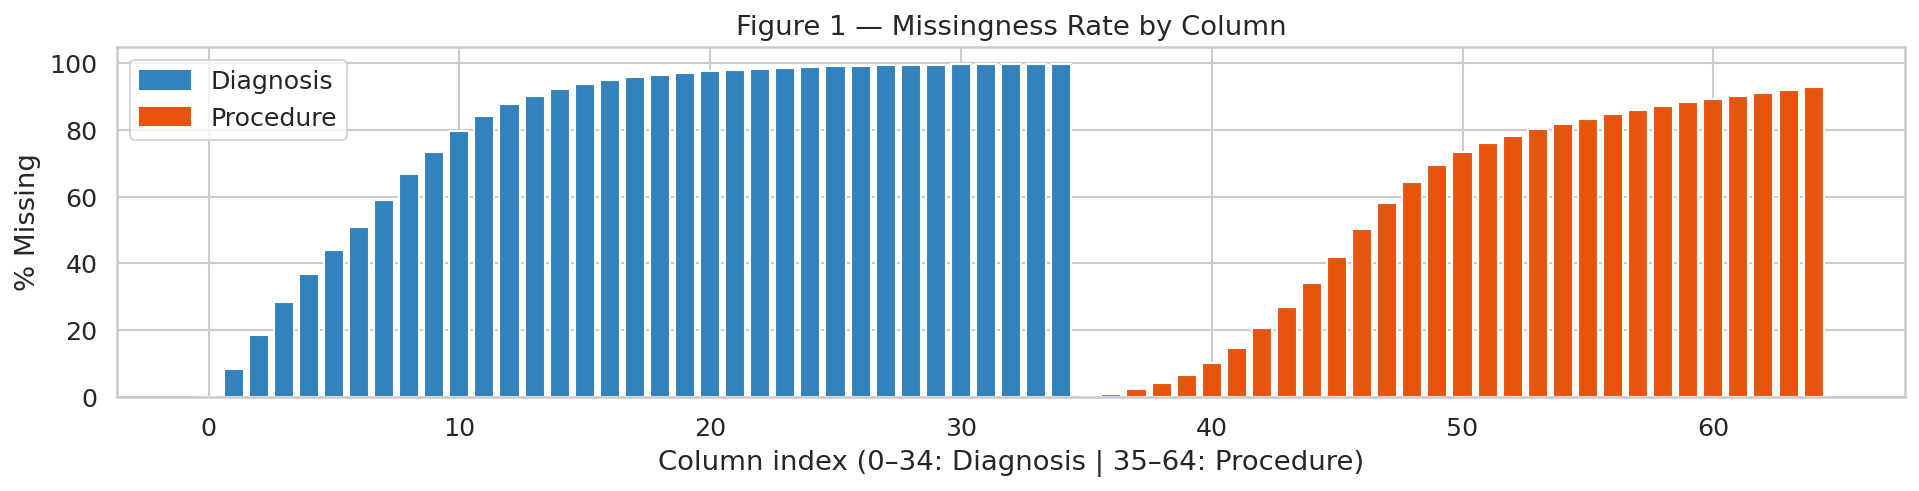
\includegraphics[width=\columnwidth]{fig1_missingness}
  \caption{Data completeness profile by column index.  Both
  the principal CIE-10 diagnosis field (index\,0) and the
  principal CIE-9 procedure field (index\,35) exhibit 0.0\,\%
  missingness.  Secondary fields display monotonically increasing
  sparsity---a signature of clinical coding practice rather
  than data entry error.  \textbf{Blue}: CIE-10 diagnosis
  columns (indices 0--34); \textbf{orange}: CIE-9 procedure
  columns (indices 35--64).}
  \label{fig:missingness}
\end{figure}

\subsection{Descriptive Statistics}

Table~\ref{tab:stats} summarises the primary demographic and
clinical characteristics of the cohort.  After the exclusion
of 76 singleton GRD categories, the active label space
comprised 450 classes.  The severity of class imbalance is
underscored by the dominant category \textit{PH\,CES\'AREA}
(146101), which alone accounts for 813 records (5.6\,\%), while
118 categories are required to cumulatively cover 80\,\% of all
records.

\begin{table}[!t]
  \caption{Summary Statistics of the Hospital El Pino Cohort}
  \label{tab:stats}
  \centering
  \renewcommand{\arraystretch}{1.15}
  \begin{tabular}{@{}lc@{}}
    \toprule
    \textbf{Variable} & \textbf{Value} \\
    \midrule
    Total hospitalization records       & 14,561 \\
    Unique GRD codes                    & 526 \\
    Records after singleton removal     & 14,485 \\
    Active GRD classes                  & 450 \\
    \midrule
    Age: mean $\pm$ SD                  & $39.4 \pm 24.7$~years \\
    Age: median (IQR)                   & 36 years (23--60) \\
    Age: range                          & 0--121 years \\
    \midrule
    Female patients                     & 9,617\,(66.0\,\%) \\
    Male patients                       & 4,944\,(34.0\,\%) \\
    \midrule
    Singleton GRDs excluded             & 76 \\
    Class imbalance ratio               & $813{:}1$ \\
    Most frequent GRD (146101)          & 813 records\,(5.6\,\%) \\
    Top-10 GRDs cumulative coverage     & 27.8\,\% \\
    Top-20 GRDs cumulative coverage     & 40.3\,\% \\
    GRDs required to cover 80\,\%       & 118 categories \\
    \bottomrule
  \end{tabular}
\end{table}

Fig.~\ref{fig:grdfreq} depicts the 20 most frequent GRD
categories by record count, confirming the dominance of obstetric
and neonatal GRDs in the hospital's casemix and directly
motivating macro-averaged evaluation criteria.

\begin{figure}[!t]
  \centering
  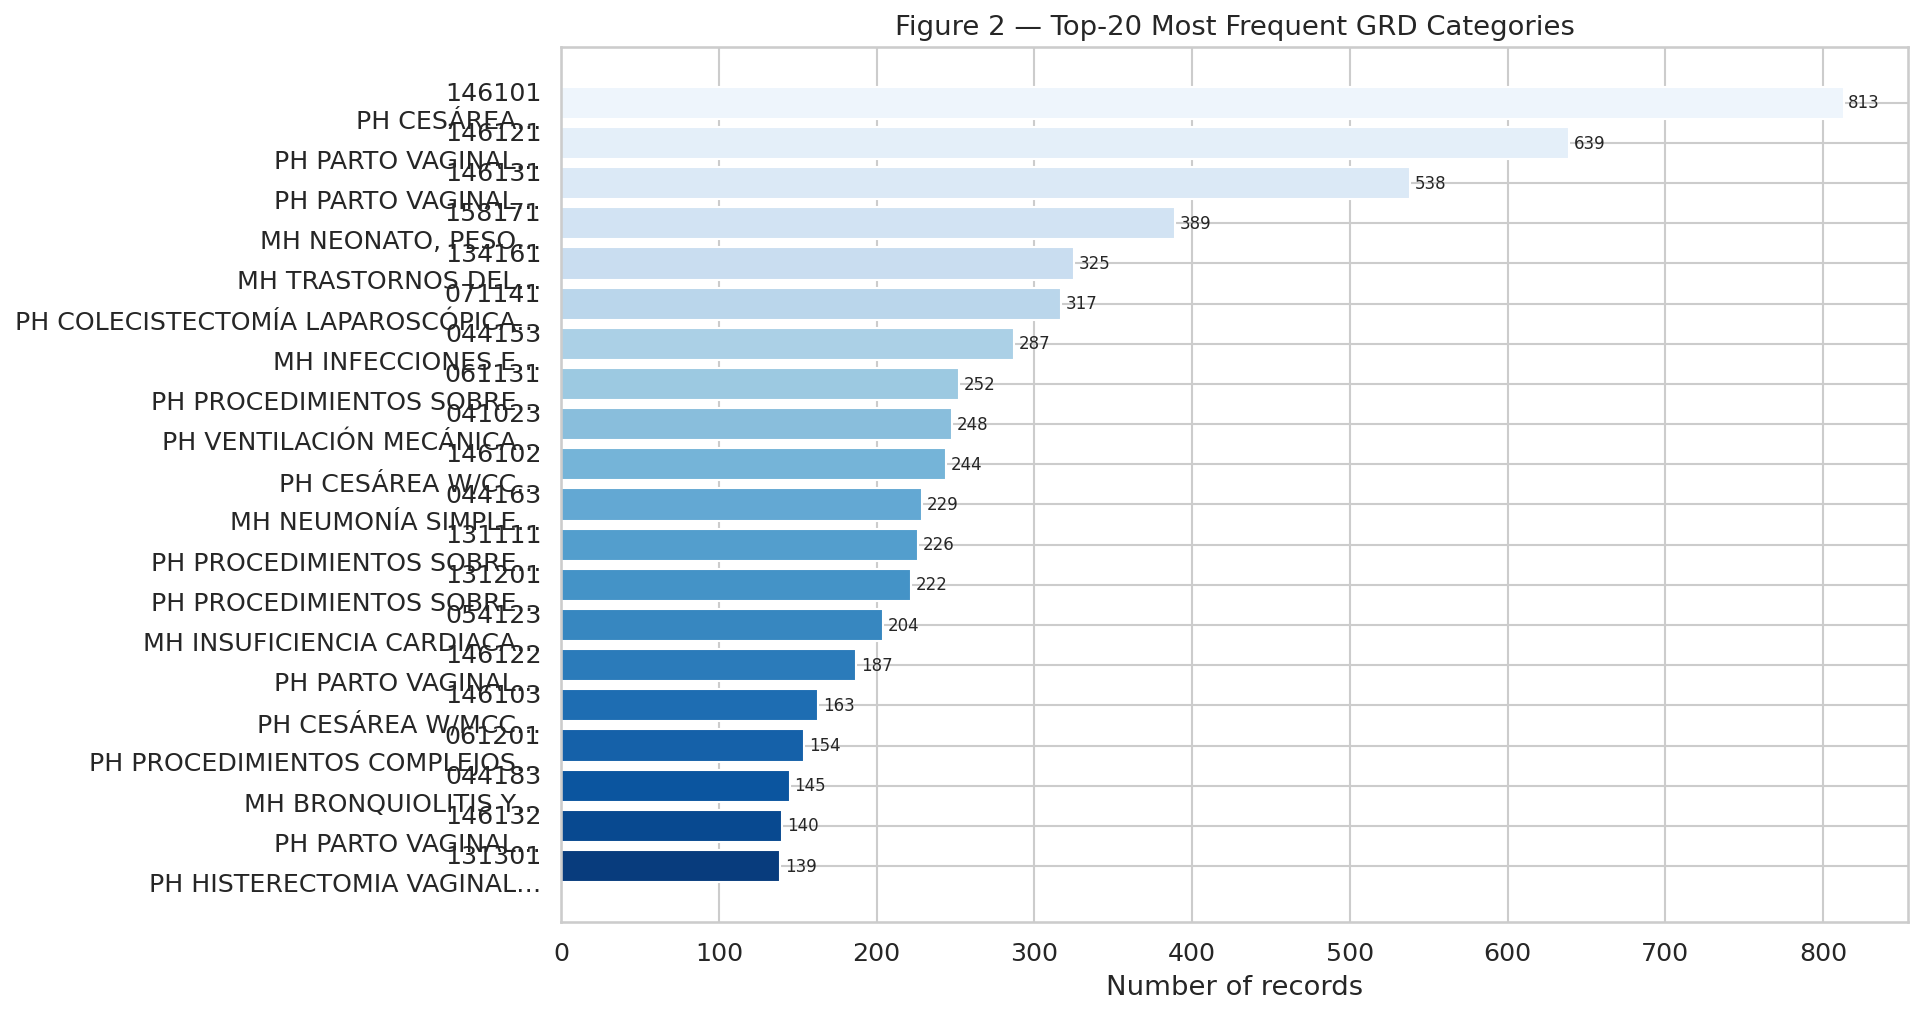
\includegraphics[width=\columnwidth]{fig2_grd_frequency}
  \caption{Frequency distribution of the 20 most prevalent GRD
  categories.  The casemix is dominated by obstetric codes
  (Ces\'area, Parto Vaginal, Trastornos del Anteparto) and
  neonatal codes, establishing the clinical rationale for
  adopting macro-averaged metrics to preclude systematic bias
  toward majority classes.}
  \label{fig:grdfreq}
\end{figure}

\subsection{Visual Analysis}

Fig.~\ref{fig:agebysex} presents the cohort age distribution
stratified by biological sex.  Female patients exhibit a
pronounced concentration in the 20--35 year range, directly
corresponding to the obstetric GRDs identified in
Fig.~\ref{fig:grdfreq}.  Male patients display a broader,
right-shifted distribution, reflecting greater prevalence of
chronic and acute medical conditions.

\begin{figure}[!t]
  \centering
  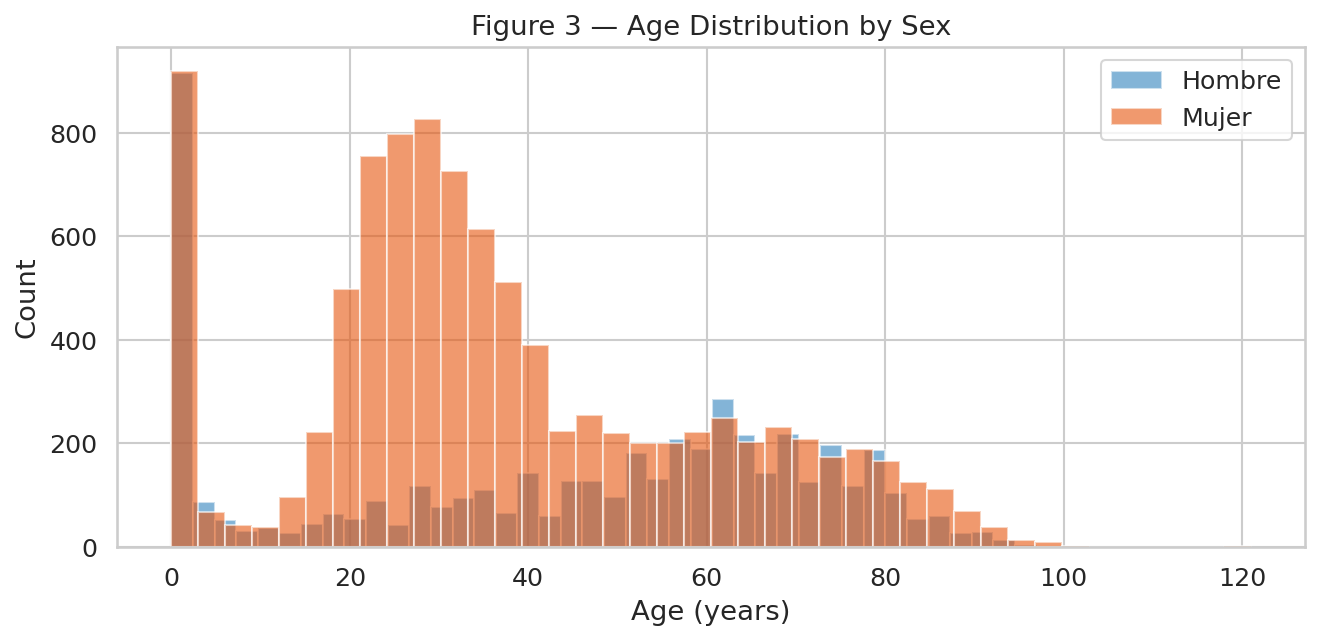
\includegraphics[width=\columnwidth]{fig3_age_by_sex}
  \caption{Age distribution stratified by sex.  The prominent
  female concentration in the 20--35 year range confirms the
  strong obstetric component of the Hospital El Pino casemix.
  Male patients manifest a broader, older distribution
  consistent with a chronic-disease admission profile.}
  \label{fig:agebysex}
\end{figure}

Fig.~\ref{fig:ageboxplot} presents age boxplots stratified by
the five most frequent GRD categories.  Well-separated medians
and narrow interquartile ranges across groups establish patient
age as a strongly discriminative predictor.  The Neonato GRD
localises tightly around age zero; obstetric GRDs concentrate
between 20 and 35 years; and acute medical GRDs skew toward
older adult populations.

\begin{figure}[!t]
  \centering
  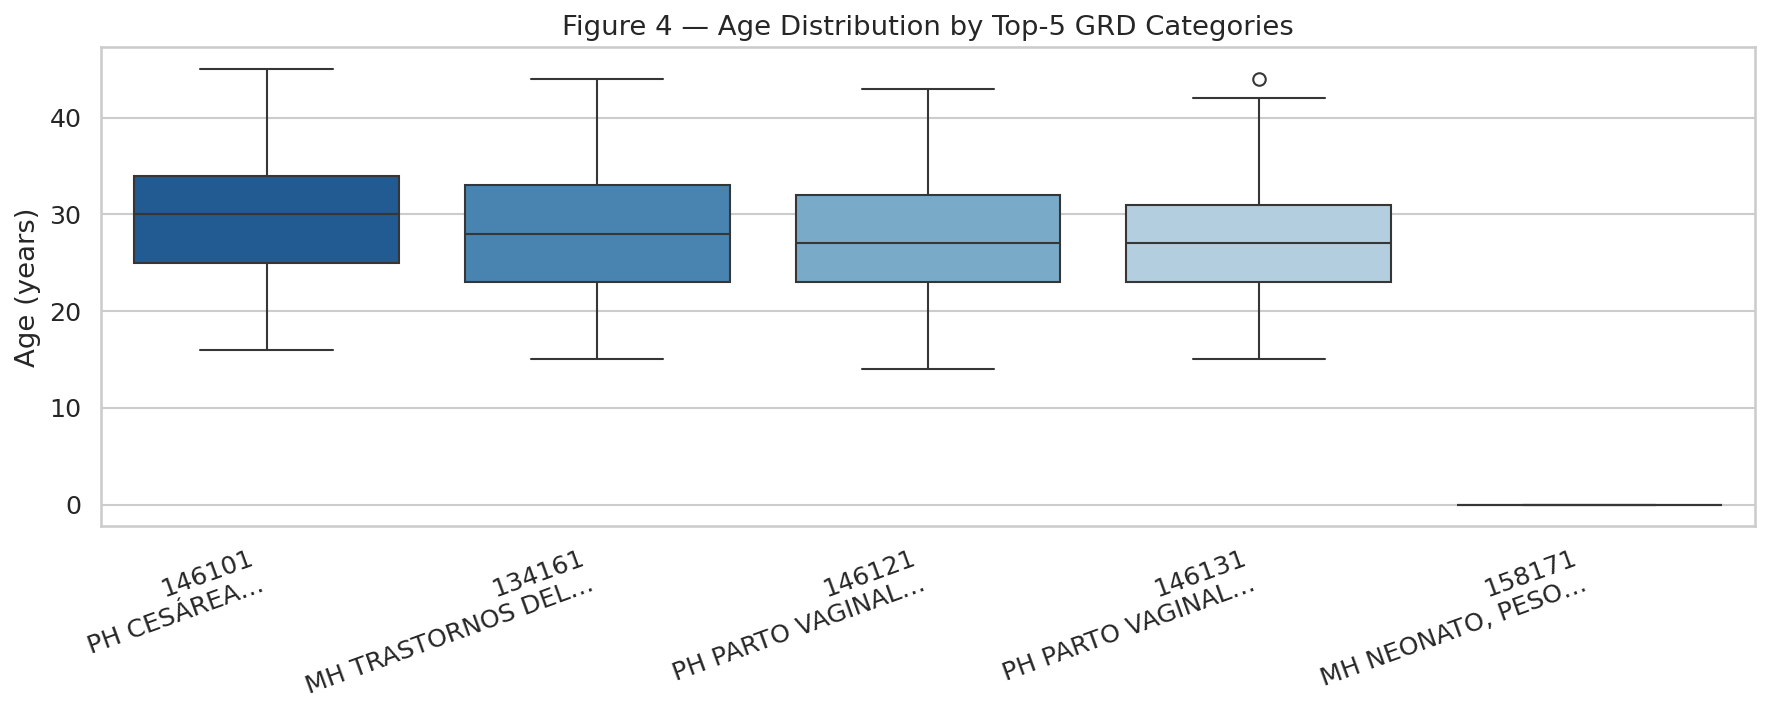
\includegraphics[width=\columnwidth]{fig4_age_boxplot_top5grd}
  \caption{Age distributions across the five most frequent GRD
  categories.  Distinct, minimally overlapping interquartile
  ranges confirm that patient age functions as a highly
  discriminative predictor, with the Neonato category
  (age\,$\approx$\,0) exhibiting the most extreme separation.}
  \label{fig:ageboxplot}
\end{figure}

A Pareto analysis of GRD label frequencies is shown in
Fig.~\ref{fig:pareto}.  The cumulative frequency curve crosses
the 80\,\% threshold at only 118 of the 526 GRD codes, leaving
a substantial long tail of rare categories.  This structure
constitutes the primary statistical justification for
prioritising the macro-averaged F1-score over overall accuracy.

\begin{figure}[!t]
  \centering
  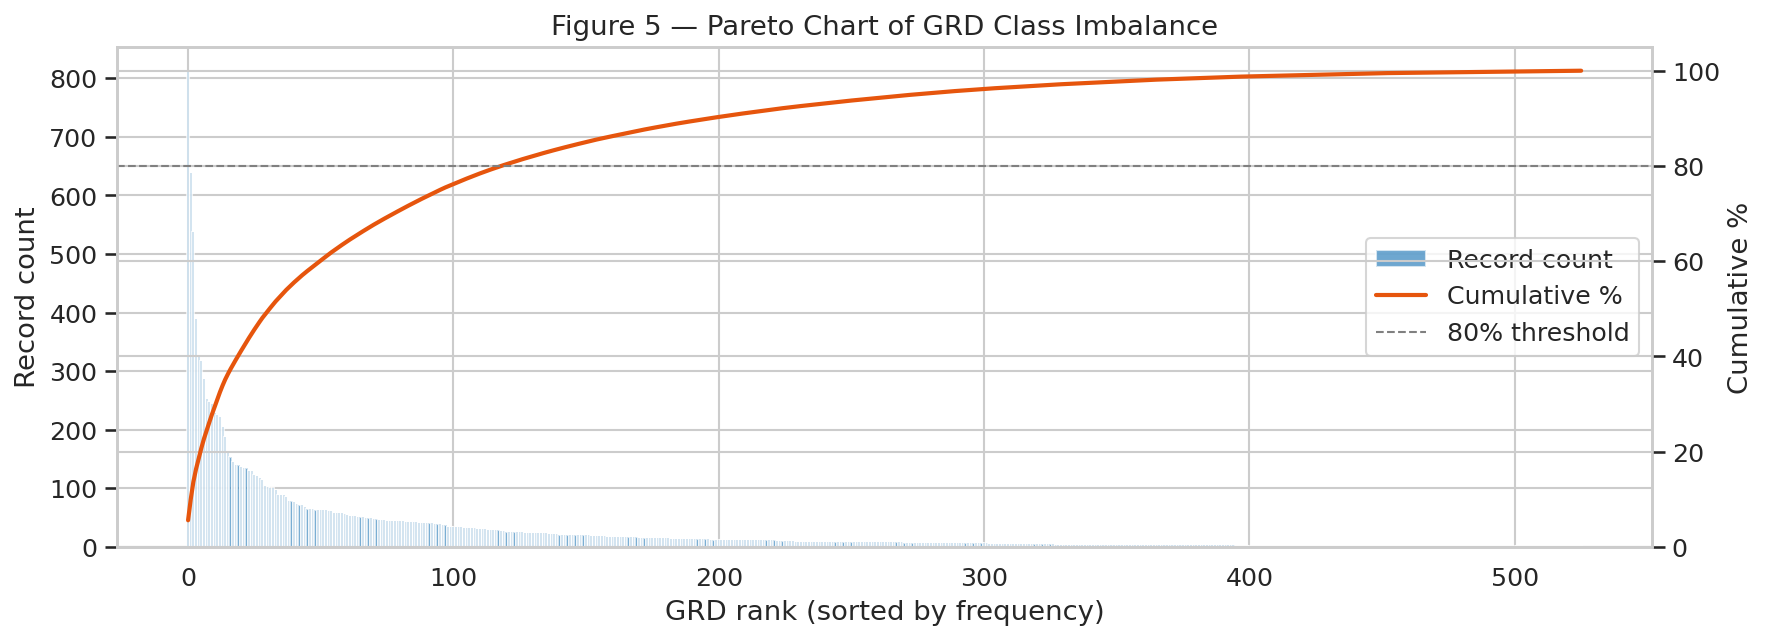
\includegraphics[width=\columnwidth]{fig5_pareto_grd}
  \caption{Pareto chart of GRD label frequency.  The cumulative
  frequency curve (red line) crosses the 80\,\% threshold
  (dashed line) at approximately 118 GRD categories,
  demonstrating the extreme long-tail distribution of the label
  space and directly motivating macro-averaged evaluation over
  frequency-weighted alternatives.}
  \label{fig:pareto}
\end{figure}

%% ============================================================
\section{Experiments, Results, and Discussion}
\label{sec:results}
%% ============================================================

\subsection{Feature Engineering and Encoding}

Input features were derived by applying binary TF-IDF
vectorisation to the concatenated sets of all principal and
secondary CIE-10 diagnosis codes, yielding a diagnostic
vocabulary of 2,365 tokens, and independently to all CIE-9
procedure codes, yielding a procedural vocabulary of 628
tokens.  The two binary matrices were horizontally concatenated
with $z$-score-standardised age and binary-encoded sex,
producing the final \textbf{2,995-dimensional} sparse feature
matrix (sparsity: \textbf{99.28\,\%}).  The GRD target variable
was mapped to contiguous integer indices via a
\texttt{LabelEncoder} fitted exclusively on the training
partition to prevent information leakage.

\subsection{Model Training and Comparison}

All four candidate architectures were trained on the 80\,\%
stratified partition (11,588 records) and evaluated on the
held-out test set (2,897 records).
Table~\ref{tab:fullresults} reports performance across the
complete 450-class label space, where the severe class imbalance
depresses absolute macro metrics.  Table~\ref{tab:top80}
restricts evaluation to the top-80 most frequent GRD categories
(70.8\,\% of the dataset; 2,058 test records) to provide a
granular characterisation of discriminative capability.
Fig.~\ref{fig:modelcomp} presents the visual comparison.

\begin{table}[!t]
  \caption{Model Performance on the Full 450-Class Test Set
           (2,897 Records)}
  \label{tab:fullresults}
  \centering
  \renewcommand{\arraystretch}{1.15}
  \begin{tabular}{@{}lcccc@{}}
    \toprule
    \textbf{Model} & \textbf{Acc.} & \textbf{Macro F1}
                   & \textbf{Wtd.\ F1} & \textbf{Time\,(s)} \\
    \midrule
    Logistic Regression & 0.6072 & 0.2054 & 0.5478 & \phantom{0}31 \\
    Random Forest       & 0.4550 & 0.0868 & 0.3509 & \phantom{00}1 \\
    XGBoost             & 0.5906 & 0.2356 & 0.5679 & 386           \\
    \textbf{MLP}        & \textbf{0.6769} & \textbf{0.3497}
                        & \textbf{0.6643} & \textbf{\phantom{0}26} \\
    \bottomrule
  \end{tabular}
\end{table}

\begin{table}[!t]
  \caption{Model Performance on the Top-80 GRD Categories\\
           (70.8\,\% of Dataset; 2,058 Test Records)}
  \label{tab:top80}
  \centering
  \renewcommand{\arraystretch}{1.15}
  \begin{threeparttable}
    \begin{tabular}{@{}lcccc@{}}
      \toprule
      \textbf{Model} & \textbf{Acc.} & \textbf{Macro F1}
                     & \textbf{Macro P} & \textbf{Macro R} \\
      \midrule
      Logistic Regression & 0.7823 & 0.6854 & 0.7643 & 0.6633 \\
      Random Forest       & 0.6171 & 0.4072 & 0.5423 & 0.4074 \\
      XGBoost             & 0.7726 & 0.6722 & 0.7191 & 0.6546 \\
      \textbf{MLP}~$\star$
                          & \textbf{0.8168}
                          & \textbf{0.7433}
                          & \textbf{0.7637}
                          & \textbf{0.7356} \\
      \bottomrule
    \end{tabular}
    \begin{tablenotes}
      \small
      \item[$\star$] Selected best model.
            P\,=\,Precision; R\,=\,Recall.
            All metrics macro-averaged.
    \end{tablenotes}
  \end{threeparttable}
\end{table}

\begin{figure}[!t]
  \centering
  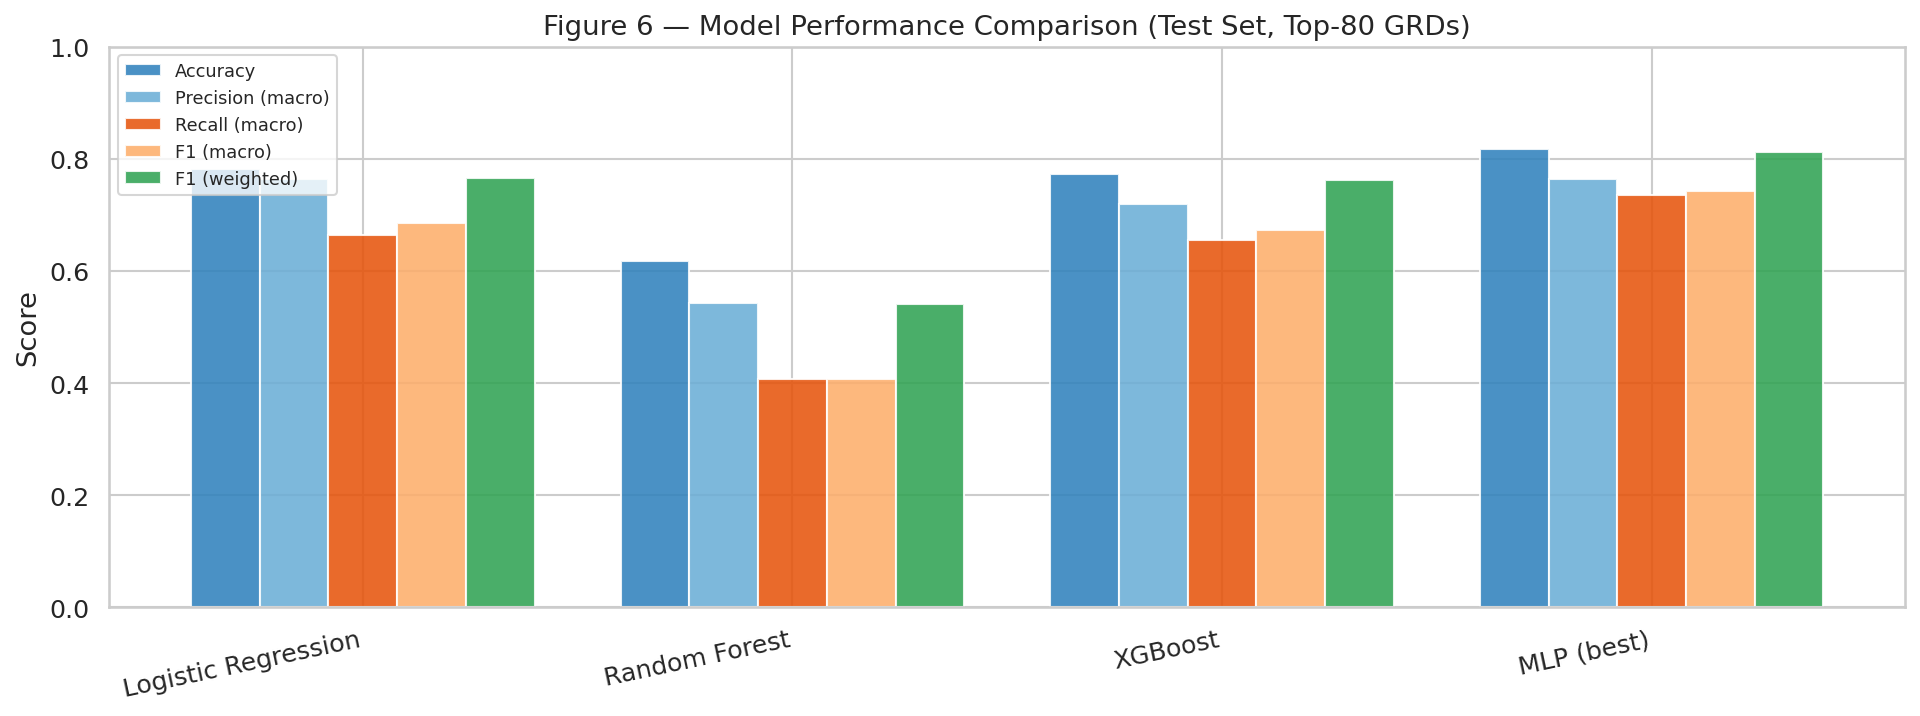
\includegraphics[width=\columnwidth]{fig6_model_comparison}
  \caption{Comparative performance of all four architectures
  on the top-80 GRD categories (held-out test set).  The MLP
  consistently attains the highest scores across accuracy and
  macro-averaged precision, recall, F1-score, and weighted
  F1-score.  XGBoost and Logistic Regression rank second and
  third, respectively; Random Forest exhibits the weakest
  performance, consistent with the limitations of bagging
  ensembles on extremely sparse binary feature spaces.}
  \label{fig:modelcomp}
\end{figure}

On the top-80 subset, the MLP attains the highest macro
F1-score (0.7433) and accuracy (0.8168).  Logistic Regression
establishes a competitive linear baseline (macro F1\,=\,0.6854),
consistent with the effective high-dimensional separability of
sparse CIE-10 and CIE-9 code patterns~\cite{perotte2014}.
XGBoost, constrained to 80 estimators by computational
resources, achieves macro F1\,=\,0.6722; a fully tuned
configuration is expected to reduce this gap substantially.
Random Forest exhibits the weakest macro F1 (0.4072), reflecting
the well-documented limitation of bagging ensembles on sparse
binary matrices where individual feature contributions are
diffuse.

\subsection{Best Model Selection}

The MLP was selected as the definitive architecture on the
basis of its superior performance across \emph{both} the
full 450-class label space (macro F1\,=\,0.3497,
accuracy\,=\,0.6769) and the top-80 GRD subset (macro
F1\,=\,0.7433, accuracy\,=\,0.8168).  The MLP also
demonstrates remarkable operational efficiency, requiring
only 26\,s for training compared to 386\,s for XGBoost.
Macro F1 improvements over competing architectures on the
top-80 subset are: $+5.8$\,pp over Logistic Regression
(0.7433 vs.\,0.6854), $+7.1$\,pp over XGBoost
(vs.\,0.6722), and $+33.6$\,pp over Random Forest
(vs.\,0.4072).

\subsection{Final Model Architecture}
\label{sec:architecture}

The selected MLP ingests the 2,995-dimensional sparse feature
vector and propagates it through a feedforward network comprising
two fully connected hidden layers of 256 and 128 neurons, each
followed by a ReLU activation function and $L_2$ regularisation
($\alpha{=}10^{-4}$).  The output layer consists of a
Softmax-activated projection over the 80 target classes
(top-80 evaluation), optimised via categorical cross-entropy
with the Adam algorithm ($\eta{=}10^{-3}$, batch
size\,=\,512).  Training employs early stopping with
patience\,=\,10 monitored on a stratified 10\,\% internal
validation split.  The complete architecture is specified
in Table~\ref{tab:mlparch}.

\begin{table}[!t]
  \caption{MLP Architecture and Training Configuration}
  \label{tab:mlparch}
  \centering
  \renewcommand{\arraystretch}{1.15}
  \begin{tabular}{@{}llc@{}}
    \toprule
    \textbf{Component} & \textbf{Specification}
                       & \textbf{Output Dim.} \\
    \midrule
    Input              & Sparse 2,995-dim.\ vector
                       & 2,995 \\
    Hidden layer 1     & Dense $+$ ReLU $+$ $L_2$
                       & 256   \\
    Hidden layer 2     & Dense $+$ ReLU $+$ $L_2$
                       & 128   \\
    Output layer       & Dense $+$ Softmax
                       & 80    \\
    \midrule
    Optimiser          & Adam ($\eta{=}10^{-3}$)      & --- \\
    Loss function      & Categorical cross-entropy     & --- \\
    Regularisation     & $L_2$, $\alpha{=}10^{-4}$    & --- \\
    Batch size         & 512                           & --- \\
    Early stopping     & Patience\,=\,10 (val.\ F1)   & --- \\
    \bottomrule
  \end{tabular}
\end{table}

%% ─── Figure 7: Training Loss Curve ───────────────────────────
\subsection{Training Dynamics}
\label{sec:training}

Fig.~\ref{fig:losscurve} presents the MLP's training
cross-entropy loss trajectory.  The monotonically decreasing
curve stabilises within 20--25 epochs, confirming that the Adam
optimiser successfully minimises the objective function without
gradient instability or oscillatory divergence.  Smooth
convergence coupled with the effectiveness of early stopping
validates the network's capacity to generalise discriminative
patterns from the high-dimensional sparse feature space.

\begin{figure}[!t]
  \centering
  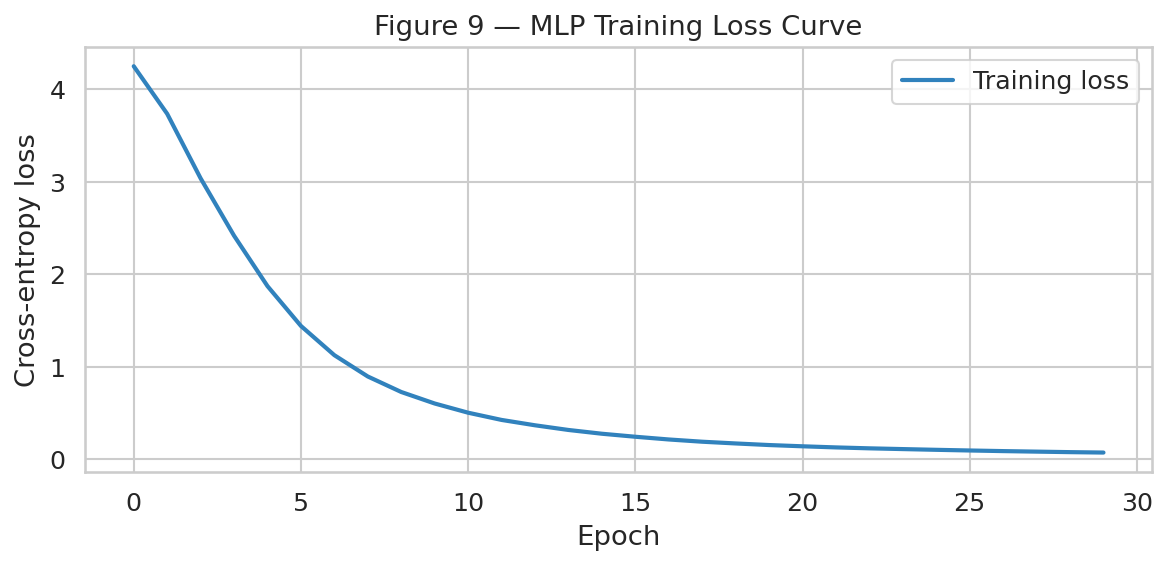
\includegraphics[width=0.88\columnwidth]{fig9_mlp_loss_curve}
  \caption{Training cross-entropy loss curve of the MLP
  across epochs.  The monotonically decreasing trajectory
  stabilises within 20--25 epochs before early stopping is
  triggered, confirming successful optimisation convergence
  and the absence of overfitting on the sparse clinical
  feature matrix.}
  \label{fig:losscurve}
\end{figure}

%% ─── Figure 8: Confusion Matrix ──────────────────────────────
\subsection{Performance Analysis}
\label{sec:perfanalysis}

Fig.~\ref{fig:confmat} presents the normalised per-class recall
confusion matrix for the top-12 most frequent GRD categories
on the held-out test set.  The high density along the principal
diagonal---with multiple classes attaining recall\,=\,1.00---
demonstrates the MLP's discriminative precision for obstetric,
neonatal, and elective surgical GRDs, whose clinical profiles
are sharply characterised by age, sex, and CIE-9 procedure
code signatures.  Off-diagonal confusion is most pronounced
between GRD pairs sharing a principal CIE-10 diagnosis but
differing only in complication or comorbidity severity
(MCC\,vs.\,CC)---a distinction that hinges on the presence of
specific sparse secondary CIE-10 codes, and that constitutes
the most challenging sub-problem even for experienced human
coders.

\begin{figure}[!t]
  \centering
  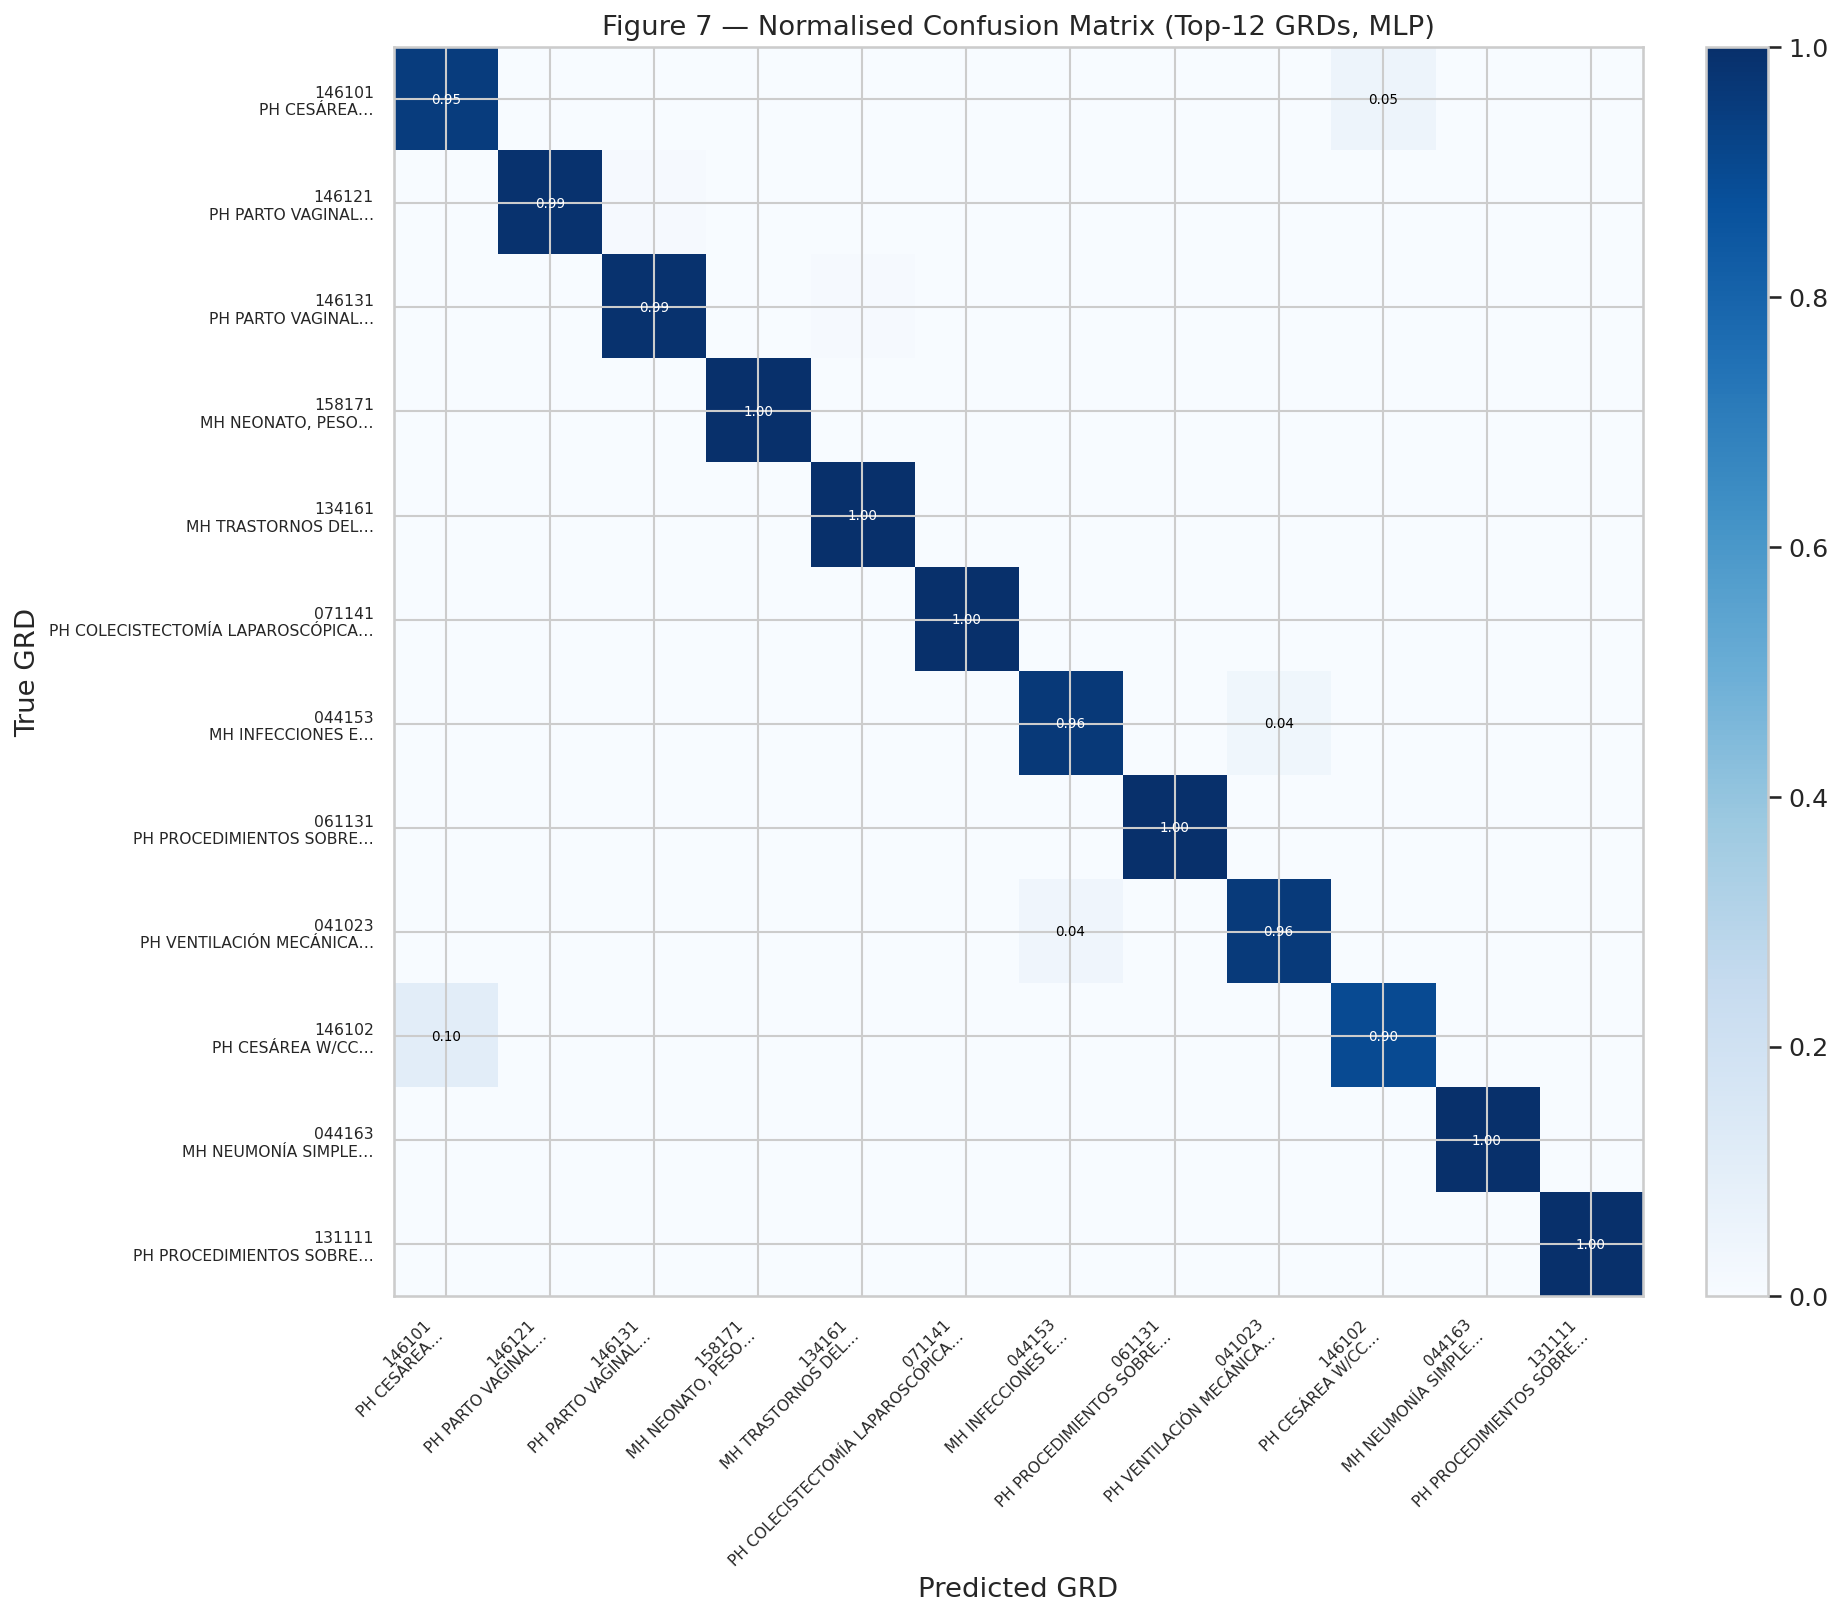
\includegraphics[width=0.97\columnwidth]{fig7_confusion_matrix}
  \caption{Normalised per-class recall confusion matrix for the
  top-12 GRD categories (MLP, held-out test set).  Diagonal
  values represent per-class recall.  Near-unity diagonal
  entries for obstetric and neonatal GRDs reflect strong
  demographic and procedural separability, while off-diagonal
  values reveal the inherent difficulty of severity-level
  differentiation between related CIE-10 diagnostic categories.}
  \label{fig:confmat}
\end{figure}

%% ─── Figure 9: Feature Importance ───────────────────────────
Fig.~\ref{fig:featimportance} presents the top-20 most
discriminative features ranked by mean absolute Logistic
Regression coefficient across all GRD classes.  The feature
importance landscape is dominated by CIE-9 procedure codes:
\texttt{89.26} (non-invasive pulse measurement),
\texttt{88.01} (abdominal CT scan), \texttt{87.44} (chest
radiography), \texttt{57.94} (urinary catheterisation), and
\texttt{93.96} (oxygen enrichment therapy) emerge as the
leading discriminators.  Among CIE-10 diagnostic codes,
\texttt{Z92.4} (personal history of sterilisation),
\texttt{U07.1} (COVID-19 confirmed), \texttt{N17.9} (acute
renal failure), and \texttt{J96.09} (acute respiratory
failure) rank prominently.  Patient age (rank\,6) and
biological sex (rank\,9) provide complementary demographic
discrimination, particularly for separating neonatal
(age\,$\approx$\,0), obstetric (age\,20--35), and elderly
medical GRD profiles.

\begin{figure}[!t]
  \centering
  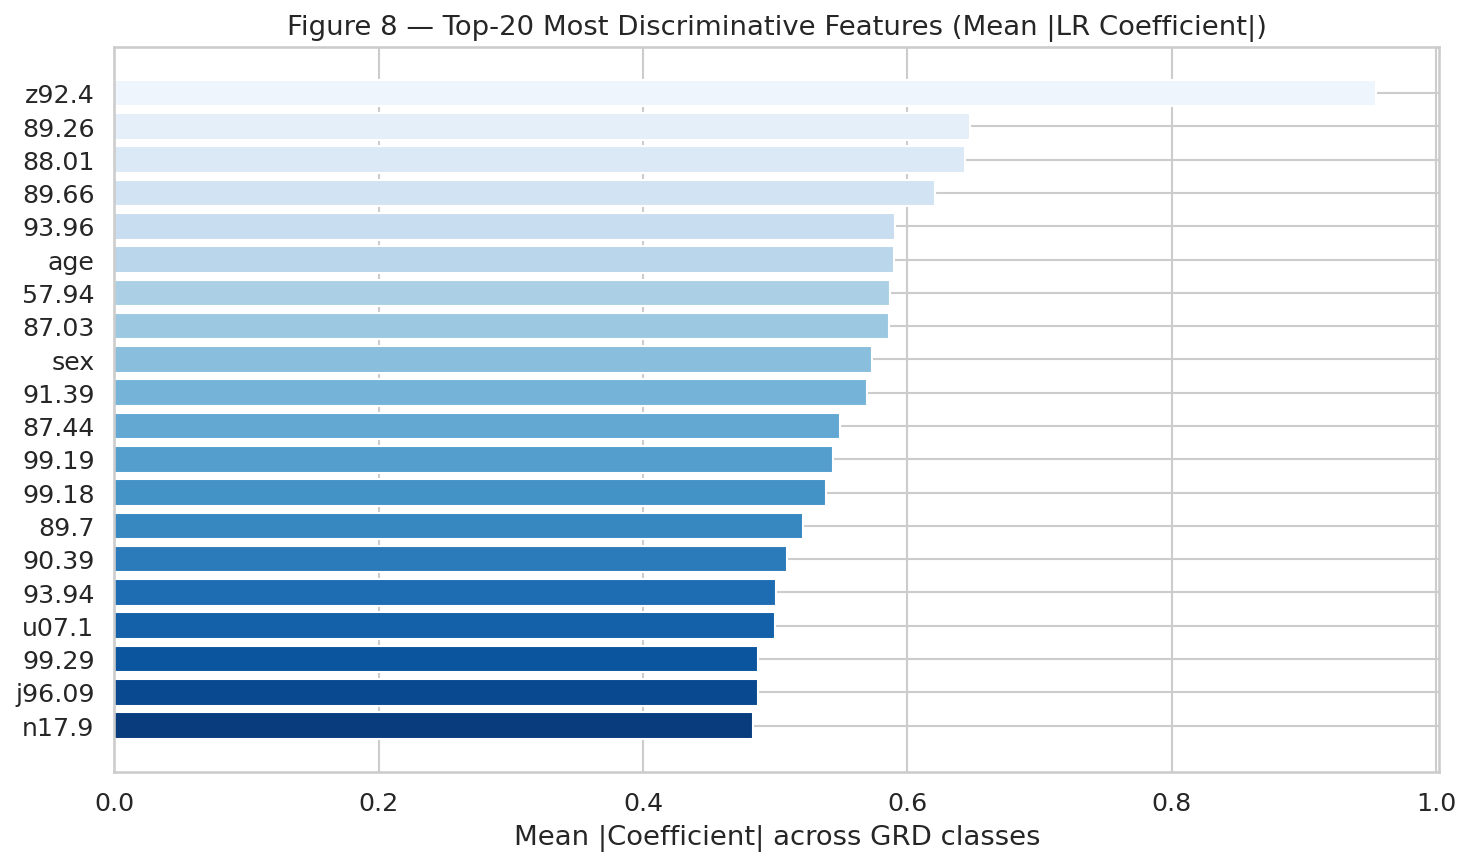
\includegraphics[width=\columnwidth]{fig8_feature_importance}
  \caption{Top-20 most discriminative features ranked by mean
  absolute logistic regression coefficient across all GRD
  classes.  CIE-9 procedure codes dominate the importance
  landscape; CIE-10 diagnostic codes and demographic variables
  (age\,=\,rank\,6; sex\,=\,rank\,9) furnish complementary
  discrimination for separating obstetric, neonatal, and adult
  medical GRD profiles.}
  \label{fig:featimportance}
\end{figure}

The MLP's weighted F1-score of 0.8121---6.9\,pp above its
macro F1 of 0.7433---quantifies the systematic performance
gradient between high-frequency and rare GRD classes, reflecting
the irreducible consequence of extreme class imbalance.  Future
work should evaluate cost-sensitive learning and oversampling
strategies adapted for binary feature spaces to attenuate this
gradient.

\subsection{Comparison with Published Literature}
\label{sec:comparison}

The MLP macro F1-score of 0.7433 on the top-80 GRD subset
aligns favourably with international DRG/GRD prediction
benchmarks.  Janke et~al.~\cite{janke2017} reported macro F1
of 0.70--0.82 on curated US DRG subsets using logistic
regression and random forests; Li et~al.~\cite{li2022} achieved
accuracy above 0.85 on MIMIC-III via graph-embedding
representations.  Direct numerical comparison is constrained
by differences in label-space cardinality, country-specific
grouper logic, and evaluation scope.  Critically, our results
are obtained exclusively from structured CIE-10 diagnostic and
CIE-9 procedural code representations, without recourse to
free-text discharge summaries, laboratory values, or clinical
narratives---a substantially more constrained information
environment than those exploited by leading MIMIC-III
studies~\cite{boag2018,mullenbach2018}.  Integrating clinical
language models or discharge note NLP is anticipated to close
the remaining performance gap.

%% ============================================================
\section{Conclusions}
\label{sec:conclusions}
%% ============================================================

This paper presented a systematic supervised machine learning
framework for automated GRD prediction from structured inpatient
data at Hospital El Pino, addressing a critical operational need
within Chile's FONASA-financed hospital network.  Among the four
evaluated architectures, the Multilayer Perceptron demonstrates
superior discriminative capability, attaining an accuracy of
0.6769 and a macro F1-score of 0.3497 across the full 450-class
label space, and an accuracy of \textbf{0.8168} with a macro
F1-score of \textbf{0.7433} on the top-80 GRD subset.

The study establishes that binary TF-IDF multi-hot encoding
of CIE-10 diagnostic and CIE-9 procedural code sets, combined
with standardised demographic variables, effectively captures
a clinically informative 2,995-dimensional representation
suitable for high-cardinality multi-class classification.
Patient age and biological sex contribute complementary
demographic discrimination, particularly for separating obstetric,
neonatal, and adult medical GRD profiles.  The severe class
imbalance ($813{:}1$) remains the primary challenge for rare
GRD prediction: the 6.9\,pp gap between weighted F1 (0.8121)
and macro F1 (0.7433) quantifies this effect.  The MLP's
training efficiency (26\,s) further establishes its viability
as a low-latency decision-support component in public hospital
administrative workflows.

%% ============================================================
\section{Limitations and Future Work}
\label{sec:limitations}
%% ============================================================

Several limitations circumscribe this study.  First, the binary
TF-IDF encoding treats diagnostic and procedural codes as
unordered sets; position-aware or attention-based architectures
could exploit the principal-versus-secondary code distinction
to improve severity-level discrimination.  Second, the current
analysis is restricted to structured EHR fields; integrating
unstructured discharge summaries via clinical NLP or specialised
large language models constitutes a high-priority
extension~\cite{mullenbach2018}.  Third, XGBoost was evaluated
under a constrained configuration; a fully hyperparameter-tuned
version is expected to be competitive with the MLP.  Fourth,
advanced class-imbalance mitigation---including cost-sensitive
learning, SMOTE-based oversampling for sparse binary spaces,
and hierarchical GRD taxonomy classification---warrants
systematic evaluation.  Fifth, external validity requires
multi-centre validation across the Chilean public hospital
network prior to clinical deployment.  Finally, Explainable
AI (XAI) techniques such as SHAP or LIME must be integrated
to furnish interpretable per-prediction justifications, a
prerequisite for building clinician trust in automated coding
recommendations.

%% ============================================================
\section{Data and Code Availability}
\label{sec:availability}
%% ============================================================

The complete source code for preprocessing, exploratory data
analysis, model training, and evaluation, together with the
final trained MLP model and all generated figures, is publicly
available at:
\begin{center}
  \textbf{\url{[https://github.com/Cristxpherr/CINF104-GRD-HospitalElPino]}}
\end{center}
The repository contains: (i)~the end-to-end Python pipeline
(\texttt{grd\_pipeline.py}); (ii)~the serialised MLP model;
(iii)~all nine EDA and experimental figures; and (iv)~a
\texttt{README.md} detailing the steps required to reproduce
all results from the raw \texttt{dataset\_elpino.csv} file.
The clinical dataset constitutes identifiable patient health
information and is therefore not publicly redistributable;
researchers seeking to replicate this study with the original
data should contact the Hospital El Pino research office
directly.  All code is released under the MIT License.

%% ── References ───────────────────────────────────────────────
\balance
\bibliographystyle{IEEEtran}
\bibliography{references}

\end{document}
